\documentclass{article}
\usepackage{fourier}
\usepackage{fullpage}
\usepackage{graphicx}
\usepackage{xspace}
\usepackage{epigraph}
\usepackage{listings}
\usepackage{xcolor}
\usepackage{url}
\usepackage{soul}
\usepackage{multirow}
\usepackage{clrscode3e}
\usepackage{hyperref}
\usepackage{wrapfig}
\usepackage{amsmath}
\usepackage{tikz}
\usetikzlibrary{calc,shapes.multipart,chains,arrows}

\title{Assignment 7\\The Great Firewall of Santa Cruz:\\Bloom Filters,
Linked Lists and Hash Tables}
\author{Prof. Darrell Long \\
CSE 13S -- Spring 2021}
\date{
  First \texttt{DESIGN.pdf} draft due: May 27$^\text{th}$ at 11:59\,pm PST \\
  Assignment (formally) due: June 4$^\text{th}$ at 11:59\,pm PST
}

\usepackage{fancyhdr}
\pagestyle{fancy}
\fancyhf{}

\fancypagestyle{plain}{%
  \fancyhf{}
  \renewcommand{\headrulewidth}{0pt}
  \renewcommand{\footrulewidth}{0pt}
  \lfoot{\textcopyright{} 2021 Darrell Long}
  \rfoot{\thepage}
}

\pagestyle{plain}

\definecolor{codegreen}{rgb}{0,0.5,0}
\definecolor{codegray}{rgb}{0.5,0.5,0.5}
\definecolor{codepurple}{rgb}{0.58,0,0.82}

\lstloadlanguages{C,make,python,fortran}

\lstdefinestyle{c99}{
    morekeywords={bool, uint8_t, uint16_t, uint32_t, uint64_t, int8_t, int16_t, int32_t, int64_t},
    commentstyle=\color{codegreen},
    keywordstyle=\color{magenta},
    numberstyle=\tiny\color{codegray},
    identifierstyle=\color{blue},
    stringstyle=\color{codepurple},
    basicstyle=\ttfamily,
    breakatwhitespace=false,
    breaklines=true,
    captionpos=b,
    keepspaces=true,
    numbers=left,
    numbersep=5pt,
    showspaces=false,
    showstringspaces=false,
    showtabs=false,
    tabsize=4
}


\begin{document}\maketitle

\section{Introduction}

\epigraphwidth=0.43\textwidth
\epigraph{\emph{War is peace. Freedom
is slavery. Ignorance is strength.}}{---George Orwell, 1984}

\noindent You have been selected through thoroughly democratic
processes (and the machinations of your friend and hero Ernst
Blofeld) to be the Dear and Beloved Leader of the Glorious People's
Republic of Santa Cruz following the failure of the short-lived
anarcho-syndicalist commune, where each person in turn acted as a
form of executive officer for the week but all the decisions of
that officer have to be ratified at a special bi-weekly meeting by
a simple majority in the case of purely internal affairs, but by a
two-thirds majority in the case of more major decisions. Where it
was understood that strange women lying in ponds distributing swords
is no basis for a system of government. Supreme executive power
derives from a mandate from the masses, not from some farcical
aquatic ceremony. It was a very silly place, and so with Herr
Blofeld's assistance you are now the leader of your people.

In order to promote virtue and prevent vice, and
to preserve social cohesion and discourage unrest, you have decided
that the Internet content must be filtered so that your beloved
children are not corrupted through the use of unfortunate, hurtful,
offensive, and far too descriptive language.


\section{Bloom Filters}

\epigraphwidth=0.75\textwidth
\epigraph{\emph{The Ministry of Peace concerns itself with war, the Ministry
of Truth with lies, the Ministry of Love with torture and the Ministry of
Plenty with starvation. These contradictions are not accidental, nor do they
result from from ordinary hypocrisy: they are deliberate exercises in
\textbf{doublethink}.}}{---George Orwell, 1984}

\noindent The Internet is very large, very fast, and full of
\emph{badthink}. The masses spend their days sending each other cat
videos and communicating through their beloved social media platforms:
Twitter and Discord. To your dismay, you find that a portion of the
masses frequently use words you deem improper---\emph{oldspeak}. You
decide, as the newly elected Dear and Beloved Leader of the Glorious
People's Republic of Santa Cruz (GPRSC), that a more neutral
\emph{newspeak} is required to keep your citizens of the GPRSC content,
pure, and from thinking too much. But how do you process and store so
many words as they flow in and out of the GPRSC at $10\,$Gbits/second?
The solution comes to your brilliant and pure mind---a \emph{Bloom
filter}.

A Bloom filter is a space-efficient probabilistic data structure,
conceived by Burton H. Bloom in 1970, and is used to test whether
an element is a member of a set. False-positive matches are possible,
but false negatives are not---in other words, a query for set membership
returns either ``possibly in the set'' or ``definitely not in the set.''
Elements can be added to the set but not removed from it; the more
elements added, the higher the probability of false positives.

\begin{wrapfigure}{r}{0.133\textwidth}
\centering

\includegraphics[width=0.12\textwidth]{images/1984-Big-Brother.jpg}
\end{wrapfigure}

A Bloom filter can be represented as an array of $m$ bits, or a
\textbf{bit vector}. A Bloom filter should utilize $k$ different hash
functions. Using these hash functions, a set element added to the Bloom
filter is mapped to at most $k$ of the $m$ bit indices, generating a
uniform pseudo-random distribution. Typically, $k$ is a small constant
which depends on the desired false error rate $\epsilon$, while $m$ is
proportional to $k$ and the number of elements to be added.

Assume you are adding a word $w$ to your Bloom filter and are using
$k=3$ hash functions, $f(x)$, $g(x)$, and $h(x)$. To add $w$ to the
Bloom filter, you simply set the bits at indices $f(w)$, $g(w)$, and
$h(w)$. To check if some word $w'$ has been added to the same Bloom
filter, you check if the bits at indices $f(w')$, $g(w')$, and $h(w')$
are set. If they are all set, then $w'$ has \emph{most likely} been
added to the Bloom filter. If any one of those bits was cleared, then
$w'$ has definitely \emph{not} been added to the Bloom filter. The fact
that the Bloom filter can only tell if some word has \emph{most likely}
been added to the Bloom filter means that \emph{false positives} can
occur. The larger the Bloom filter, the lower the chances of getting
false positives.

So what do Bloom filters mean for you as the Dear and Beloved Leader?
It means you can take a list of proscribed words, \emph{oldspeak} and
add each word into your Bloom filter. If any of the words that your
citizens use seem to be added to the Bloom filter, then this is very
ungood and further action must be taken to discern whether or not the
citizen did transgress. You decide to implement a Bloom filter with
\emph{three} salts for \emph{three} different
hash functions. Why? To reduce the chance of a \emph{false positive}.

You can think of a ``salt'' as an initialization vector or a key. Using
different salts with the same hash function results in a different,
unique hash. Since you are equipping your Bloom filter with three
different salts, you are effectively getting three different hash
functions: $f(x)$, $g(x)$, and $h(x)$. Hashing a word $w$, with
extremely high probability, should result in $f(w) \ne g(w) \ne h(w)$.
These salts are to be used for the SPECK cipher, which requires a
128-bit key, so we have used MD5 \footnote{Rivest, R.. “The MD5
  Message-Digest Algorithm.” RFC 1321 (1992): 1-21.} ``message-digest''
  to reduce three books down to 128 bits each. You will use the SPECK
  cipher as a hash function, which will be discussed in \S 4.

\subsection{\texttt{BloomFilter}}

The following \texttt{struct} defines the \texttt{BloomFilter} ADT. The
three salts will be stored in the \texttt{primary}, \texttt{secondary},
and \texttt{tertiary} fields. Each salt is 128 bits in size. To hold
these 128 bits, we use an array of two \texttt{uint64\_t}s. This
\texttt{struct} definition \emph{must} go in \texttt{bf.c}.

\begin{codelisting}{}
struct BloomFilter {
  uint64_t primary[2];   // Primary hash function salt.
  uint64_t secondary[2]; // Secondary hash function salt.
  uint64_t tertiary[2];  // Tertiary hash function salt.
  BitVector *filter;
};
\end{codelisting}

\subsection{\texttt{BloomFilter *bf\_create(uint32\_t size)}}

The constructor for a Bloom filter. Working code for the constructor,
complete with primary, secondary, and tertiary salts that you will use,
is shown below. Note that you will also have to implement the bit vector
ADT for your Bloom filter, as it will serve as the array of bits
necessary for a proper Bloom filter.

\begin{codelisting}{}
BloomFilter *bf_create(uint32_t size) {
  BloomFilter *bf = (BloomFilter *) malloc(sizeof(BloomFilter));
  if (bf) {
    // Grimm's Fairy Tales
    bf->primary[0] = 0x5adf08ae86d36f21;
    bf->primary[1] = 0xa267bbd3116f3957;
    // The Adventures of Sherlock Holmes
    bf->secondary[0] = 0x419d292ea2ffd49e;
    bf->secondary[1] = 0x09601433057d5786;
    // The Strange Case of Dr. Jekyll and Mr. Hyde
    bf->tertiary[0] = 0x50d8bb08de3818df;
    bf->tertiary[1] = 0x4deaae187c16ae1d;
    bf->filter = bv_create(size);
    if (!bf->filter) {
      free(bf);
      bf = NULL;
    }
  }
  return bf;
}
\end{codelisting}

\subsection{\texttt{void bf\_delete(BloomFilter **bf)}}

The destructor for a Bloom filter. As with all other destructors, it
should free any memory allocated by the constructor and null out the
pointer that was passed in.

\subsection{\texttt{uint32\_t bf\_size(BloomFilter *bf)}}

Returns the size of the Bloom filter. In other words, the number of bits
that the Bloom filter can access. Hint: this is the length of the
underlying bit vector.

\subsection{\texttt{void bf\_insert(BloomFilter *bf, char *oldspeak)}}

Takes \texttt{oldspeak} and inserts it into the Bloom filter. This
entails hashing \texttt{oldspeak} with each of the three salts for three
indices, and setting the bits at those indices in the underlying bit
vector.

\subsection{\texttt{bool bf\_probe(BloomFilter *bf, char *oldspeak)}}

Probes the Bloom filter for \texttt{oldspeak}. Like with
\texttt{bf\_insert()}, \texttt{oldspeak} is hashed with each of the
three salts for three indices. If all the bits at those indices are set,
return \texttt{true} to signify that \texttt{oldspeak} was most likely
added to the Bloom filter. Else, return \texttt{false}.

\subsection{\texttt{uint32\_t bf\_count(BloomFilter *bf)}}

Returns the number of set bits in the Bloom filter.

\subsection{\texttt{void bf\_print(BloomFilter *bf)}}

A debug function to print out a Bloom filter.

\section{Hashing with the SPECK Cipher}

You will need a good hash function to use in your Bloom filter and hash
table (discussed in \S 5). We will have discussed hash functions in
lecture, and rather than risk having a poor one implemented, we will
simply provide you one. The SPECK\footnote{ Ray Beaulieu, Stefan
  Treatman-Clark, Douglas Shors, Bryan Weeks, Jason Smith, and Louis
Wingers, ``The {SIMON} and {SPECK} lightweight block ciphers.'' In
Proceedings of the 52nd ACM/EDAC/IEEE Design Automation Conference
(DAC), pp.  1--6. IEEE, 2015.} block cipher is provided for use as a
hash function.

SPECK is a family of lightweight block ciphers publicly released by the
National Security Agency (NSA) in June 2013.  SPECK has been optimized
for performance in software implementations, while its sister algorithm,
SIMON, has been optimized for hardware implementations. SPECK is an
add-rotate-xor (ARX) cipher. The reason a cipher is used for this is
because encryption generates random output given some input; exactly
what we want for a hash.

Encryption is the process of taking some file you wish to protect,
usually called plaintext, and transforming its data such that only
authorized parties can access it. This transformed data is referred to
as ciphertext. Decryption is the inverse operation of encryption, taking
the ciphertext and transforming the encrypted data back to its original
state as found in the original plaintext. Encryption algorithms that
utilize the same key for both encryption and decryption, like SPECK, are
symmetric-key algorithms, and algorithms that don't, such as RSA, are
asymmetric-key algorithms.

You will be given two files, \texttt{speck.h} and \texttt{speck.c}. The
former will provide the interface to using the SPECK hash function which
has been named \texttt{hash()}, and the latter contains the
implementation. The hash function \texttt{hash()} takes two parameters:
a 128-bit salt passed in the form of an array of two
\texttt{uint64\_t}s, and a key to hash. The function will return a
\texttt{uint32\_t} which is exactly the index the key is mapped to.

\begin{codelisting}{}
uint32_t hash(uint64_t salt[], char *key);
\end{codelisting}{}

\section{Bit Vectors}

\epigraph{\emph{Symmetrical equations are good in their place, but `vector'
is a useless survival, or offshoot from quaternions, and has never been of the
slightest use to any creature.}}{---Lord Kelvin}

\noindent You will reuse much of the bit vector implementation from assignment 5
for this assignment. If there were any problems with your
implementation, make sure to fix them here.

\begin{codelisting}{}
struct BitVector {
  uint32_t length;
  uint8_t *vector;
};
\end{codelisting}

\subsection{\texttt{BitVector *bv\_create(uint32\_t length)}}

The constructor for a bit vector. In the even that sufficient memory
cannot be allocated, the function must return \texttt{NULL}. Else, it
must return a \texttt{BitVector *)}, or a pointer to an allocated
\texttt{BitVector}. Each bit of the bit vector should be initialized to
0.

\subsection{\texttt{void bv\_delete(BitVector **bv)}}

The destructor for a bit vector. Remember to set the pointer to
\texttt{NULL} after the memory associated with the bit vector is freed.

\subsection{\texttt{uint32\_t bv\_length(BitVector *bv)}}

Returns the length of a bit vector.

\subsection{\texttt{void bv\_set\_bit(BitVector *bv, uint32\_t i)}}

Sets the $i^\text{th}$ bit in a bit vector. To set a bit in a bit
vector, it is necessary to first locate the byte in which the
$i^\text{th}$ resides. The location of the byte is calculated as
\texttt{i / 8}. The position of the bit in that byte is calculated as
\texttt{i \% 8}. Setting a bit in a bit vector should not modify any of
the other bits.

\subsection{\texttt{void bv\_clr\_bit(BitVector *bv, uint32\_t i)}}

Clears the $i^\text{th}$ bit in the bit vector.

\subsection{\texttt{uint8\_t bv\_get\_bit(BitVector *bv, uint32\_t i)}}

Returns the $i^\text{th}$ bit in the bit vector.

\subsection{\texttt{void bv\_print(BitVector *bv)}}

A debug function to print a bit vector. \textcolor{red}{Write this
immediately after the constructor}.


\section{Hash Tables}

\epigraph{\emph{To send men to the firing squad, judicial proof is
unnecessary \ldots These procedures are an archaic bourgeois
detail.}}{Ernesto Ch\'e Guevara}

\noindent Armed with a Bloom filter, you now exercise the power to catch and
punish those who practice wrongthink and continue to use oldspeak. It
comes to mind however, that a Bloom filter is probabilistic and that it
is better to exercise mercy and counsel the oldspeakers so that they may
atone and use \emph{newspeak}. To remedy this, another solution pops
into your brilliant and pure mind---a \emph{hash table}.

\begin{wrapfigure}{r}{0.133\textwidth}
\centering

\includegraphics[width=0.130\textwidth]{images/Blofeld.png}
\end{wrapfigure}

A hash table is a data structure that maps keys to values and provides
fast, $\operatorname{O}(1)$, look-up times. It does so typically by
taking a key $k$, hashing it with some hash function $h(x)$, and placing
the key's corresponding value in an underlying array at index $h(k)$.
This is the perfect way not only to store translations from oldspeak to
newspeak, but also as a way to store all prohibited oldspeak words
without newspeak translations. We will refer to oldspeak without
newspeak translations as \emph{badspeak}. So what happens when two
\emph{oldspeak} words have the same hash value?  This is called a
\emph{hash collision}, and must be resolved. Rather than doing
\emph{open addressing} (as will be discussed in lecture), we will be
using \emph{linked lists} to resolve \emph{oldspeak} hash collisions.


\subsection{\texttt{HashTable}}

Below is the \texttt{struct} definition for a hash table. Similar to a
Bloom filter, a hash table contains a salt which is passed to
\texttt{hash()} whenever a new oldspeak entry is being inserted. As
mentioned in \S 5, we will be using linked lists to resolve oldspeak
hash collisions, which is why a hash table contains an array of linked
lists. The \texttt{mtf} field indicates whether or not the linked
lists should use the \emph{move-to-front} technique, which will be
discussed in \S 5.6.

\begin{codelisting}{}
struct HashTable {
  uint64_t salt[2];
  uint32_t size;
  bool mtf;
  LinkedList **lists;
};
\end{codelisting}

\subsection{\texttt{HashTable *ht\_create(uint32\_t size, bool mtf)}}

The constructor for a hash table. The \texttt{size} parameter denotes
the number of indices, or linked lists, that the hash table can index up
to. The salt for the hash table has been supplied in the constructor as
well.

\begin{codelisting}{}
HashTable *ht_create(uint32_t size, bool mtf) {
  HashTable *ht = (HashTable *) malloc(sizeof(HashTable));
  if (ht) {
    // Leviathan
    ht->salt[0] = 0x9846e4f157fe8840;
    ht->salt[1] = 0xc5f318d7e055afb8;
    ht->size = size;
    ht->mtf = mtf;
    ht->lists = (LinkedList **) calloc(size, sizeof(LinkedList *));
    if (!ht->lists) {
      free(ht);
      ht = NULL;
    }
  }
  return ht;
}
\end{codelisting}

\subsection{\texttt{void ht\_delete(HashTable **ht)}}

The destructor for a hash table. Each of the linked lists in
\texttt{lists}, the underlying array of linked lists, is freed.
The pointer that was passed in should be set to \texttt{NULL}.

\subsection{\texttt{uint32\_t ht\_size(HashTable *ht)}}

Returns the hash table's size.

\subsection{\texttt{Node *ht\_lookup(HashTable *ht, char *oldspeak)}}

Searches for an entry, a node, in the hash table that contains
\texttt{oldspeak}. A node stores oldspeak and its newspeak translation.
The index of the linked list to perform a look-up on is calculated by
hashing the \texttt{oldspeak}. If the node is found, the pointer to the
node is returned. Else, a \texttt{NULL} pointer is returned.

\subsection{\texttt{void ht\_insert(HashTable *ht, char *oldspeak,
char *newspeak)}}

Inserts the specified \texttt{oldspeak} and its corresponding
\texttt{newspeak} translation into the hash table. The index of the
linked list to insert into is calculated by hashing the
\texttt{oldspeak}. If the linked list that should be inserted into
hasn't been initialized yet, create it first before inserting the
oldspeak and newspeak.

\subsection{\texttt{uint32\_t ht\_count(HashTable *ht)}}

Returns the number of non-\texttt{NULL} linked lists in the hash table.

\subsection{\texttt{void ht\_print(HashTable *ht)}}

A debug function to print out the contents of a hash table. \textcolor{red}{Write this
immediately after the constructor}.

\section{Linked Lists}

\epigraph{\emph{Education is a weapon, whose effect depends on who holds
it in his hands and at whom it is aimed.}}{---Joseph Stalin}

\noindent A \emph{linked list} will be used to resolve hash collisions.
Each node of the linked list contains \emph{oldspeak} and its
\emph{newspeak} translation if it exists. The \emph{key} to search with
in the linked list is \emph{oldspeak}. Each node will also contain a
pointer to the previous node \emph{and} the next node in the linked
list. This is because you will be implementing \emph{doubly linked
lists}.

\subsection{\texttt{Node}}

A node is defined with the following \texttt{struct}:

\begin{codelisting}{}
struct Node {
  char *oldspeak;
  char *newspeak;
  Node *next;
  Node *prev;
};
\end{codelisting}

If the \texttt{newspeak} field is \texttt{NULL}, then the oldspeak
contained in this node is badspeak, since there is no newspeak
translation. This \texttt{struct} definition and interface for the node
ADT will be provided for you in \texttt{node.h}. The node ADT is not
opaque in order to simplify the rest of the linked list implementation.

\subsection{\texttt{Node *node\_create(char *oldspeak, char *newspeak)}}

The constructor for a node. You will want to make a \emph{copy} of the
\texttt{oldspeak} and its \texttt{newspeak} translation that are passed
in. What this means is \emph{allocating memory} and copying over the
characters for both \texttt{oldspeak} and \texttt{newspeak}. There was a
function \texttt{strdup()} that did precisely that, but it has been
deprecated. You will find it helpful to implement your own function to
mimic \texttt{strdup()}.

\subsection{\texttt{void node\_delete(Node **n)}}

The destructor for a node. Only the node \texttt{n} is freed. The
previous and next nodes that \texttt{n} points to \emph{are not}
deleted. Since you have allocated memory for \texttt{oldspeak} and
\texttt{newspeak}, remember to free the memory allocated to both of
those as well. The pointer to the node should be set to \texttt{NULL}.

\subsection{\texttt{void node\_print(Node *n)}}

While helpful as debug function, you will use this function to produce
correct program output. Thus, it is imperative that you print out the
contents of a node in the following manner:

\begin{itemize}
  \item If the node \texttt{n} contains oldspeak \emph{and} newspeak,
    print out the node with this print statement:
    \begin{codelisting}{}
printf("%s -> %s\n", n->oldspeak, n->newspeak);
    \end{codelisting}
  \item If the node \texttt{n} contains \emph{only} oldspeak, meaning
    that newspeak is null, then print out the node with this print
    statement:
    \begin{codelisting}{}
printf("%s\n", n->oldspeak);
    \end{codelisting}
\end{itemize}

\subsection{\texttt{LinkedList}}

The \texttt{struct} definition of a linked list is given below. A
linked list, when constructed, will initially have two \emph{sentinel}
nodes, which will be further explained in \S 6.6 where the constructor
function is discussed along with the rationale and usage of the sentinel
nodes. The field \texttt{mtf} signifies the \emph{move-to-front}
technique, which will be further explained in \S 6.6 and \S 6.10. The
linked list interface, defined in \texttt{ll.h}, will contain the
declaration of two \texttt{extern} variables: \texttt{seeks} and
\texttt{links}. \textcolor{red}{These two variables should be defined in
\texttt{ll.c}.} You will use these variables to calculate statistics,
where \texttt{seeks} tracks the number of linked list lookups performed,
and \texttt{links} counts the total number of links traversed.

\begin{codelisting}{}
struct LinkedList {
  uint32_t length;
  Node *head; // Head sentinel node.
  Node *tail; // Tail sentinel node.
  bool mtf;
};
\end{codelisting}

\subsection{\texttt{LinkedList *ll\_create(bool mtf)}}

The constructor for a linked list. The only parameter that this function
takes is a boolean, \texttt{mtf}. If \texttt{mtf} is \texttt{true}, that
means any node that is found in the linked list through a look-up is
\emph{moved to the front} of the linked list. To simplify the code to
insert nodes into the linked list, your linked lists will be initialized
with exactly two \emph{sentinel nodes}. They will serve as the head and
the tail of the linked list.

A linked list that is not initialized with sentinel nodes exhibits two
different cases when inserting a node. The first case is when the linked
list is empty and contains no nodes. This means the inserted node
becomes the head of the linked list. The second case is when the linked
list contains at least one node, which means the inserted node becomes
the new head of the linked list and must point to the old head of the
linked list. The old head of the linked list must also point back to the
new head to preserve the properties of a doubly linked list.

Using two sentinel nodes reduces the insertion cases down to one: every
inserted node will go between two nodes. Why? Because there are already
two nodes to start with. The following diagrams showcase, in order, a
linked list when initialized, the linked list when a node containing
\texttt{x} is inserted, and then the linked list when a node containing
\texttt{y} is inserted. Note that inserting a node into a linked list
means inserting it \emph{at the head}.

\begin{center}
  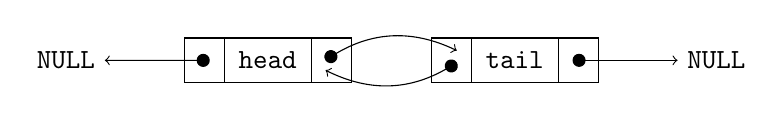
\begin{tikzpicture}[
      list/.style={
            rectangle split,
            rectangle split parts=3, draw,
            rectangle split horizontal,
            inner sep=5pt, text=black
        },
        ->, start chain
      ]
    \node[list,on chain] (A) {\nodepart{second} \texttt{head}};
    \node[list,on chain] (C) {\nodepart{second} \texttt{tail}};

    \node (D) [right=of C] {\texttt{NULL}};
    \node (E) [left= of A] {\texttt{NULL}};

    \path[*->] let \p1 = (A.three), \p2 = (A.center) in
    (\x1,\y2) edge [bend left] ($(C.one)+(0.15,0.2)$);

    \draw[*->] let \p1 = (C.three), \p2 = (C.center) in (\x1,\y2) -- (D);
    \draw[*->] ($(A.one)+(0.15,0.075)$) -- (E);

    \path[*->] ($(C.one)+(0.15,0.05)$) edge [bend left] ($(A.three)+(0,-0.05)$);
  \end{tikzpicture}
\end{center}

\begin{center}
  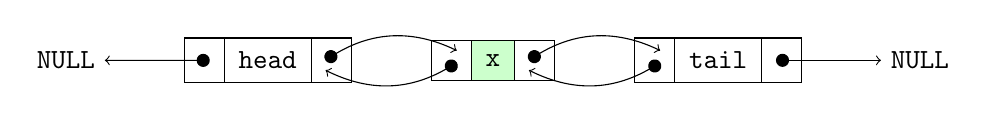
\begin{tikzpicture}[
      list/.style={
            rectangle split,
            rectangle split parts=3, draw,
            rectangle split horizontal,
            inner sep=5pt, text=black
        },
      new/.style={
            rectangle split,
            rectangle split parts=3, draw,
            rectangle split horizontal,
            inner sep=5pt, text=black,
            rectangle split part fill={white, green!20, white}
        },
      ->, start chain
      ]
    \node[list,on chain] (A) {\nodepart{second} \texttt{head}};
    \node[new,on chain] (B) {\nodepart{second} \texttt{x}};
    \node[list,on chain] (C) {\nodepart{second} \texttt{tail}};
    \node (D) [right=of C] {\texttt{NULL}};
    \node (E) [left= of A] {\texttt{NULL}};

    \path[*->] let \p1 = (A.three), \p2 = (A.center) in
    (\x1,\y2) edge [bend left] ($(B.one)+(0.15,0.2)$);

    \path[*->] let \p1 = (B.three), \p2 = (B.center) in
    (\x1,\y2) edge [bend left] ($(C.one)+(0.15,0.2)$);

    \draw[*->] let \p1 = (C.three), \p2 = (C.center) in (\x1,\y2) -- (D);

    \draw[*->] ($(A.one)+(0.15,0.075)$) -- (E);
    \path[*->] ($(B.one)+(0.15,0.05)$) edge [bend left] ($(A.three)+(0,-0.05)$);
    \path[*->] ($(C.one)+(0.15,0.05)$) edge [bend left] ($(B.three)+(0,-0.05)$);
  \end{tikzpicture}
\end{center}

\begin{center}
  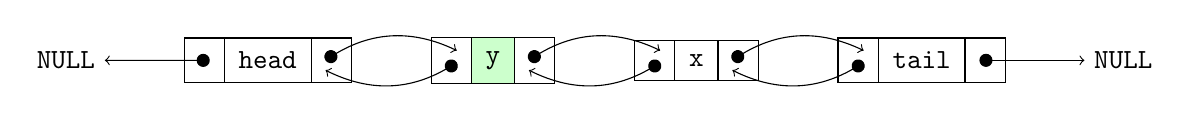
\begin{tikzpicture}[
      list/.style={
            rectangle split,
            rectangle split parts=3, draw,
            rectangle split horizontal,
            inner sep=5pt, text=black
        },
      new/.style={
            rectangle split,
            rectangle split parts=3, draw,
            rectangle split horizontal,
            inner sep=5pt, text=black,
            rectangle split part fill={white, green!20, white}
        },
      ->, start chain
      ]
    \node[list,on chain] (A) {\nodepart{second} \texttt{head}};
    \node[new,on chain] (F) {\nodepart{second} \texttt{y}};
    \node[list,on chain] (B) {\nodepart{second} \texttt{x}};
    \node[list,on chain] (C) {\nodepart{second} \texttt{tail}};
    \node (D) [right=of C] {\texttt{NULL}};
    \node (E) [left= of A] {\texttt{NULL}};

    \path[*->] let \p1 = (A.three), \p2 = (A.center) in
    (\x1,\y2) edge [bend left] ($(F.one)+(0.15,0.2)$);

    \path[*->] let \p1 = (F.three), \p2 = (F.center) in
    (\x1,\y2) edge [bend left] ($(B.one)+(0.15,0.2)$);

    \path[*->] let \p1 = (B.three), \p2 = (B.center) in
    (\x1,\y2) edge [bend left] ($(C.one)+(0.15,0.2)$);

    \draw[*->] let \p1 = (C.three), \p2 = (C.center) in (\x1,\y2) -- (D);

    \draw[*->] ($(A.one)+(0.15,0.075)$) -- (E);
    \path[*->] ($(F.one)+(0.15,0.05)$) edge [bend left] ($(A.three)+(0,-0.05)$);
    \path[*->] ($(B.one)+(0.15,0.05)$) edge [bend left] ($(F.three)+(0,-0.05)$);
    \path[*->] ($(C.one)+(0.15,0.05)$) edge [bend left] ($(B.three)+(0,-0.05)$);
  \end{tikzpicture}
\end{center}

\subsection{\texttt{void ll\_delete(LinkedList **ll)}}

The destructor for a linked list. Each node in the linked list should be
freed using \texttt{node\_delete()}. The pointer to the linked list
should be set to \texttt{NULL}.

\subsection{\texttt{uint32\_t ll\_length(LinkedList *ll)}}

Returns the length of the linked list, which is equivalent to the number
of nodes in the linked list, \emph{not} including the head and tail
sentinel nodes.

\subsection{\texttt{Node *ll\_lookup(LinkedList *ll, char
*oldspeak)}}

Searches for a node containing \texttt{oldspeak}. If a node is found,
the pointer to the node is returned. Else, a \texttt{NULL} pointer is
returned. If a node was found and the move-to-front option was specified
when constructing the linked list, then the found node is moved to the
front of the linked list. The move-to-front technique decreases look-up
times for nodes that are frequently searched for. You will learn more
about optimality in your future classes.

\subsection{\texttt{void ll\_insert(LinkedList *ll, char *oldspeak,
char *newspeak)}}

Inserts a new node containing the specified \texttt{oldspeak} and
\texttt{newspeak} into the linked list. Before inserting the node, a
look-up is performed to make sure the linked list \emph{does not} already
contain a node containing a matching \texttt{oldspeak}. If a duplicate
exists, a new node is not inserted into the linked list. Else, the new
node is inserted \emph{at the head} of the linked list. This means
that the new node comes directly after the head sentinel node.

\subsection{\texttt{void ll\_print(LinkedList *ll)}}

Prints out each node in the linked list \emph{except} for the head and
tail sentinel nodes. This will require the use of
\texttt{node\_print()}.


\section{Lexical Analysis with Regular Expressions}

\epigraphwidth=0.5\textwidth
\epigraph{\emph{Ideas are more powerful than guns. We would not let our
enemies have guns, why should we let them have ideas.}}{---Joseph
Stalin}

Back to regulating your citizens of the GPRSC. You will need a function
to parse out the words that they speak, which will be passed to you in
the form of an input stream. The words that they will use are valid
words, which can include \emph{contractions} and \emph{hyphenations}.
A valid word is any sequence of one or more characters that are part of
your regular expression word character set. Your word character set
should contain characters from a--z, A--Z, 0--9, and the underscore
character. Since you also accept contractions like ``don't'' and
``y'all've'' and hyphenations like ``pseudo-code'' and
``move-to-front'', your word character set should include apostrophes
and hyphens as well.

You will need to write your own \emph{regular expression} for a word,
utilizing the \texttt{regex.h} library to lexically analyze the input
stream for words. You will be given a parsing module that lexically
analyzes the input stream using your regular expression. You are not
required to use the module itself, but it is \emph{mandatory} that you
parse through an input stream for words using at least one regular
expression. The interface for the parsing module will be in
\texttt{parser.h} and its implementation will be in \texttt{parser.c}.

The function \texttt{next\_word()} requires two inputs, the input stream
\texttt{infile}, and a pointer to a compiled regular expression,
\texttt{word\_regex}. Notice the word \emph{compiled}: you must first compile
your regular expression using \texttt{regcomp()} before passing it to the
function. Make sure you remember to call the function \texttt{clear\_words()} to
free any memory used by the module when you're done reading in words.
Here is a small program that prints out words input to \texttt{stdin}
using the parsing module. In the program, the regular expression for a
word matches one or more lowercase and uppercase letters. The regular
expression you will have to write for your assignment will be more
complex than the one displayed here, as it is just an example.

\begin{codelisting}{Example program using the parsing module.}
#include "parser.h"
#include <regex.h>
#include <stdio.h>

#define WORD "[a-zA-Z]+"

int main(void) {
    regex_t re;
    if (regcomp(&re, WORD, REG_EXTENDED)) {
        fprintf(stderr, "Failed to compile regex.\n");
        return 1;
    }

    char *word = NULL;
    while ((word = next_word(stdin, &re)) != NULL) {
        printf("Word: %s\n", word);
    }

    clear_words();
    regfree(&re);
    return 0;
}
\end{codelisting}


\section{Your Task}

\epigraphwidth=0.5\textwidth
\epigraph{\emph{The people will believe what the media tells them they
believe.}}{---George Orwell}

\begin{itemize}
  \item Initialize your Bloom filter and hash table.
  \item Read in a list of \emph{badspeak} words with \texttt{fscanf()}.
    Again, badspeak is simply oldspeak without a newspeak translation.
    Badspeak is strictly forbidden. Each badspeak word should be added
    to the Bloom filter and the hash table. The list of proscribed words
    will be in \texttt{badspeak.txt}, which can be found in the
    \texttt{resources} repository.
  \item Read in a list of \emph{oldspeak} and \emph{newspeak} pairs with
    \texttt{fscanf()}. Only the oldspeak should be added to the Bloom
    filter. The oldspeak \emph{and} newspeak are added to the hash
    table. The list of oldspeak and newspeak pairs will be in
    \texttt{newspeak.txt}, which can also be found in the
    \texttt{resources} repository.
  \item Now that the lexicon of badspeak and oldspeak/newspeak
    translations has been populated, you can start to filter out words.
    Read words in from \texttt{stdin} using the supplied parsing module.
  \item For each word that is read in, check to see if it has been added
    to the Bloom filter. If it has not been added to the Bloom filter,
    then no action is needed since the word isn't a proscribed word.
  \item If the word has most likely been added to the Bloom filter,
    meaning \texttt{bf\_probe()} returned \texttt{true}, then further
    action needs to be taken.
    \begin{enumerate}
      \item If the hash table contains the word and the word \emph{does
        not} have a newspeak translation, then the citizen who used this
        word is guilty of \texttt{thoughtcrime}. Insert this badspeak
        word into a list of badspeak words that the citizen used in
        order to notify them of their errors later.
      \item If the hash table contains the word, and the word \emph{does}
        have a newspeak translation, then the citizen requires
        counseling on proper \emph{Rightspeak}. Insert this oldspeak
        word into a list of oldspeak words with newspeak translations in
        order to notify the citizen of the revisions needed to be made
        in order to practice Rightspeak.
      \item If the hash table does not contain the word, then all is
        good since the Bloom filter issued a false positive. No
        disciplinary action needs to be taken.
    \end{enumerate}
  \item If the citizen is accused of thoughtcrime \emph{and} requires
    counseling on proper \emph{Rightspeak}, then they are given a
    reprimanding \emph{mixspeak message} notifying them of their
    transgressions and promptly sent off to \emph{joycamp}. The message
    should contain the list of badspeak words that were used followed by
    the list of oldspeak words that were used with their proper newspeak
    translations.

    \begin{lstlisting}[style=plainstyle]
    Dear beloved citizen of the GPRSC,

    We have some good news, and we have some bad news.
    The good news is that there is bad news. The bad news is that you will
    be sent to joycamp and subjected to a week-long destitute existence.
    This is the penalty for using degenerate words, as well as using
    oldspeak in place of newspeak. We hope you can correct your behavior.

    Your transgressions, followed by the words you must think on:

    kalamazoo
    antidisestablishmentarianism
    write -> papertalk
    sad -> happy
    read -> papertalk
    music -> noise
    liberty -> badfree\end{lstlisting}

  \item If the citizen is accused solely of thoughtcrime, then they are
    issued a thoughtcrime message and also sent off to \emph{joycamp}.
    The \emph{badspeak message} should contain the list of badspeak
    words that were used.

  \begin{lstlisting}[style=plainstyle]
    Dear beloved citizen of the GPRSC,

    You have been caught using degenerate words that may cause
    distress among the moral and upstanding citizens of the GPSRC.
    As such, you will be sent to joycamp. It is there where you will
    sit and reflect on the consequences of your choice in language.

    Your transgressions:

    kalamazoo
    antidisestablishmentarianism\end{lstlisting}

  \item If the citizen only requires counseling, then they are issued an
    encouraging \emph{goodspeak message}. They will read it, correct
    their \emph{wrongthink}, and enjoy the rest of their stay in the
    GPRSC. The message should contain the list of oldspeak words that
    were used with their proper newspeak translations.

    \begin{lstlisting}[style=plainstyle]
    Dear beloved citizen of the GPRSC,

    We recognize your efforts in conforming to the language standards
    of the GPSRC. Alas, you have been caught uttering questionable words
    and thinking unpleasant thoughts. You must correct your wrongspeak
    and badthink at once. Failure to do so will result in your deliverance
    to joycamp.

    Words that you must think on:

    write -> papertalk
    sad -> happy
    read -> papertalk
    music -> noise
    liberty -> badfree\end{lstlisting}

  \item Each of the messages are defined for you in \texttt{messages.h}.
    \textcolor{red}{You may not modify this file}.

  \item The list of the command-line options your program must support
    is listed below. \emph{Any} combination of the command-line options
    must be supported.
    \begin{itemize}
      \item \texttt{-h} prints out the program usage. Refer to the
      reference program in the resources repository for what to print.
      \item \texttt{-t size} specifies that the hash table
        will have \texttt{size} entries (the default will be $10000$).
      \item \texttt{-f size} specifies that the Bloom filter
        will have \texttt{size} entries (the default will be $2^{20}$).
      \item \texttt{-m} will enable the \emph{move-to-front rule}. By
        default, the move-to-front rule is \emph{disabled}.
      \item \texttt{-s} will enable the printing of statistics to
        \texttt{stdout}. The statistics to calculate are the total
        number of seeks, the average seek length, the hash table load,
        and the Bloom filter load. The calculations for the latter three
        statistics are as follows:
        \begin{align*}
          \text{Average seek length} &=
          \frac{\texttt{links}}{\texttt{seeks}} \\
          \text{Hash table load} &= 100 \times \frac{\texttt{ht\_count()}}{\texttt{ht\_size()}} \\
          \text{Bloom filter load} &= 100 \times \frac{\texttt{bf\_count()}}{\texttt{bf\_size()}}
        \end{align*}
        The hash table load and Bloom filter load should be printed with
        up to 6 digits of precision. \textcolor{red}{Enabling the
        printing of statistics should \emph{suppress all messages} the
      program may otherwise print.}
    \end{itemize}
\end{itemize}


\section{Deliverables}

\epigraph{\emph{I would rather have questions that can't be answered than
answers that can't be questioned.}}{---Richard P. Feynman}

You will need to turn in:

\begin{enumerate}
  \item \texttt{banhammer.c}: This contains \texttt{main()} and
    \emph{may} contain the other functions necessary to complete the
    assignment.
  \item \texttt{messages.h}: Defines the mixspeak, badspeak, and
    goodspeak messages that are used in \texttt{banhammer.c}.
    \textcolor{red}{Do not modify this.}
  \item \texttt{speck.h}: Defines the interface for the hash function
    using the SPECK cipher. \textcolor{red}{Do not modify this.}
  \item \texttt{speck.c}: Contains the implementation of the hash
    function using the SPECK cipher. \textcolor{red}{Do not modify this.}
  \item \texttt{ht.h}: Defines the interface for the hash table ADT.
    \textcolor{red}{Do not modify this.}
  \item \texttt{ht.c}: Contains the implementation of the hash table
    ADT.
  \item \texttt{ll.h}: Defines the interface for the linked list ADT.
    \textcolor{red}{Do not modify this.}
  \item \texttt{ll.c}: Contains the implementation of the linked list
    ADT.
  \item \texttt{node.h}: Defines the interface for the node ADT.
    \textcolor{red}{Do not modify this.}
  \item \texttt{node.c}: Contains the implementation of the node ADT.
  \item \texttt{bf.h}: Defines the interface for the Bloom filter ADT.
    \textcolor{red}{Do not modify this.}
  \item \texttt{bf.c}: Contains the implementation of the Bloom filter ADT.
  \item \texttt{bv.h}: Defines the interface for the bit vector ADT.
    \textcolor{red}{Do not modify this.}
  \item \texttt{bv.c}: Contains the implementation of the bit vector
    ADT.
  \item \texttt{parser.h}: Defines the interface for the regex parsing
    module. \textcolor{red}{Do not modify this.}
  \item \texttt{parser.c}: Contains the implementation of the regex
    parsing module.
  \item You may have other source and header files, but \emph{do not
    make things overly complicated}.

  \item \texttt{Makefile}: This is a file that will allow the grader to
    type \texttt{make} to compile your program.

    \begin{itemize}
      \item \texttt{CC=clang} must be specified.
      \item \texttt{CFLAGS=-Wall -Wextra -Werror -Wpedantic}
        must be included.
      \item \texttt{make} should build the \texttt{banhammer}
        executable, as should \texttt{make all}.
      \item \texttt{make clean} must remove all files that are compiler
        generated.
      \item \texttt{make format} should format all your source code,
        including the header files.
    \end{itemize}

  \item Your code must pass \texttt{scan-build} \emph{cleanly}. If there
    are any bugs or errors that are false positives, document them and
    explain why they are false positives in your \texttt{README.md}.

  \item \texttt{README.md}: This must be in Markdown. This must describe
    how to use your program and \texttt{Makefile}. This includes listing
    and explaining the command-line options that your program accepts.
    Any false positives reported by \texttt{scan-build} should go here
    as well.

  \item \texttt{DESIGN.pdf}: This \emph{must} be a PDF. The design
    document should describe your design for your program with enough
    detail that a sufficiently knowledgeable programmer would be able to
    replicate your implementation. This does not mean copying your
    entire program in verbatim. You should instead describe how your
    program works with supporting pseudocode. For this program, pay
    extra attention to how you build each necessary component.

  \item \texttt{WRITEUP.pdf}: This document \emph{must} be a PDF. The
    writeup must include the following:
    \begin{itemize}
      \item Graphs comparing the total number of seeks and average seek
        length as you vary the hash table and Bloom filter size.
        \begin{itemize}
          \item Do linked lists get longer?
          \item How does the number of links followed without using the
            move-to-front rule compare to the number of links followed
            using the rule?
          \item How does changing the Bloom filter size affect the
            number of lookups performed in the hash table?
        \end{itemize}
      \item Analysis of the graphs you produce.
    \end{itemize}
\end{enumerate}


\section{Submission}

\epigraph{\emph{We can and must write in a language which sows among the
masses hate, revulsion, and scorn toward those who disagree with
us.}}{---Vladimir Lenin}

\noindent To submit your assignment through \texttt{git}, refer to the
steps shown in \texttt{asgn0} Remember: \emph{add, commit,} and
\emph{push}! \textcolor{red}{Your assignment is turned in \emph{only}
  after you have pushed and submitted the commit ID to Canvas. Your
  design document is turned in \emph{only} after you have pushed and
  submitted the commit ID to Canvas. If you forget to push, you have
  not turned in your assignment and you will get a \emph{zero}. ``I
forgot to push'' is not a valid excuse. It is \emph{highly} recommended
to commit and push your changes \emph{often}.}

\section{Supplemental Readings}

\epigraph{\emph{The more you read, the more things you will know. The
more that you learn, the more places you'll go.}}{---Dr.\ Seuss}\noindent

\begin{itemize}
  \item \textit{The C Programming Language} by Kernighan \& Ritchie
  \begin{itemize}
    \item Chapter 5 \S 5.7
    \item Chapter 7
  \end{itemize}
  \item \textit{Introduction to Algorithms} by T.\ Cormen, C.\
    Leiserson, R.\ Rivest, \& C.\ Stein
    \begin{itemize}
      \item Chapter 10 \S 10.2 (Linked lists)
      \item Chapter 11 (Hash tables and hash functions)
    \end{itemize}
  \item \textit{Introduction to the Theory of Computation} by M.\ Sipser
    \begin{itemize}
      \item Chapter 1 \S 1.3 (Regular expressions)
    \end{itemize}
\end{itemize}

\begin{center}
  
\includegraphics[width=0.35\textwidth]{../../images/monkey-chainsaw.jpg} \\
  \vspace{10pt}
  % ROT13 cipher.
  % Laugh now while you can, monkey-boy.
  \texttt{Ynhtu abj juvyr lbh pna, zbaxrl-obl.}
\end{center}

\end{document}
